\chapter{Objects}
\label{Chp:Objects}

The GraphBLAS \emph{algebraic objects} operators, monoids, and semirings
are presented below.
These objects can be used as input arguments to various GraphBLAS
operations, as shown in Table~\ref{Tab:OperatorInputType}.
The specific rules for each algebraic object
are explained in the respective sections of those objects.  A summary
of the properties and recipes for building these GraphBLAS algebraic
objects is presented in Table~\ref{Tab:AlgebraicObjects}.

\begin{table}
    \hrule
    \begin{center}
        \caption{Operator input for relevant GraphBLAS operations. 
        The semiring add and times are shown if applicable.\scott{Kronecker Changes}}
        \label{Tab:OperatorInputType}
        \begin{tabular}{l|l}
        Operation           			& Operator input  	\\ \hline
        {\sf mxm, mxv, vxm} 			& semiring 		\\ \hline
        {\sf eWiseAdd}      			& binary operator   	\\
                            			& monoid           	\\
                            			& semiring          	\\ \hline
        {\sf eWiseMult}     			& binary operator   	\\
                            			& monoid          	\\
                            			& semiring         	\\ \hline
       {\sf reduce} (to vector)  		& binary operator	\\ 
                            			& monoid           	\\ \hline
       {\sf reduce} (to scalar)  		& monoid           	\\ \hline
       {\sf apply}         			    & unary operator   	\\ \hline
       {\sf kronecker}                  & binary operator   	\\
                            			& monoid           	\\
                            			& semiring          	\\ \hline
       {\sf dup} argument (build methods)  	& binary operator   	\\ \hline
       {\sf accum} argument (various methods) 	& binary operator  	\\
       \end{tabular}
    \end{center}
    \hrule
\end{table}

\begin{table}
	\hrule
	\begin{center}
		\caption{Properties and recipes for building GraphBLAS algebraic objects: unary operator, binary operator, monoid, and semiring (composed of operations \emph{add} and \emph{times}).\newline
		\hspace{\textwidth}Note 1: The output domain of the semiring times must be same as the domain of the semiring add. This ensures three domains for a semiring rather than four.}
		\label{Tab:AlgebraicObjects}
		
		\vspace{1\baselineskip}
		(a) Properties of algebraic objects.
		\vspace{1\baselineskip}
		
		\begin{tabular}{l|l|l|l|l}
			Object 		& Must be  	& Must be  	& Identity 	& Number \\
			       		& commutative 	& associative 	& must exist 	& of domains  \\
            \hline
			Unary operator 	& no		& no		& no 		& 2 \\
			Binary operator & no		& no 		& no 		& 3  \\
			Monoid          & no		& yes 		& yes 		& 1  \\
			Semiring add 	& yes		& yes 		& yes  		& 1  \\
			Semiring times 	& no		& no 		& no 		& 3  (see Note 1) \\
		\end{tabular}
		
		\vspace{1\baselineskip}
		(b) Recipes for algebraic objects.
		\vspace{1\baselineskip}
		
		\begin{tabular}{l|l|l}
			Object          & Recipe                			            & Number of domains  \\ 
                        \hline
			Unary operator  & Function pointer      			            & 2 \\				
			Binary operator & Function pointer      			            & 3  \\	
			Monoid          & Associative binary operator with identity 	& 1  \\
			Semiring        & Commutative monoid $+$ binary operator 	    & 3 \\
		\end{tabular}
		
	\end{center}
	\hrule
\end{table}

Once algebraic objects (operators, monoids, and semirings) are described,
we introduce \emph{collections} (vectors, matrices, and masks) that
algebraic objects operate on. Finally, we introduce \emph{descriptors},
which are a simple way to modify how algebraic objects operate on
collections. More concretely, descriptors can be used (among other
things) to perform multiplication with transpose of matrix without the
user having to manually transpose the collection. A complete list of
what descriptors are capable of can be found in the section.

Every GraphBLAS object has a \emph{lifetime}, which consists of
the sequence of instructions executed in program order between the
\emph{creation} and the \emph{destruction} of the object.  Pre-defined
objects (types, operators, monoids, semirings and descriptors) are created
when the GraphBLAS context is initialized by a call to {\sf GrB\_init}
and are destroyed when the GraphBLAS context is terminated by a call to
{\sf GrB\_finalize}.

Additional objects can be created by a call to a \emph{constructor}.
Each kind of object has its own explicit constructor method: {\sf GrB\_Type\_new},
{\sf GrB\_UnaryOp\_new}, {\sf GrB\_BinaryOp\_new}, {\sf GrB\_Monoid\_new},
{\sf GrB\_Semiring\_new}, {\sf GrB\_Descriptor\_new}, {\sf GrB\_Vector\_new},
{\sf GrB\_Matrix\_new}. Furthermore, vectors and matrices can be
constructed by duplicating another vector or matrix through calls 
to the methods {\sf GrB\_Vector\_dup} and {\sf GrB\_Matrix\_dup}, respectively.
Objects explicitly created by a call to a constructor can be destroyed
by a call to {\sf GrB\_free}. The behavior of a program
that calls {\sf GrB\_free} on a pre-defined object is undefined.

Several GraphBLAS constructor methods take objects as input arguments
and use these objects to create a new object. For all {\sf GrB\_*\_new}
methods, the lifetime of the created object must end strictly before
the lifetime of any input objects. For example, a vector constructor
{\sf GrB\_Vector\_new} takes a type object as input. That type
object must not be destroyed until after the created vector is destroyed.
Similarly, a {\sf GrB\_Semiring\_new} method takes a monoid and
a binary operator as inputs. Neither of these can be destroyed until
after the created semiring is destroyed.

The {\sf GrB\_Vector\_dup} and {\sf GrB\_Matrix\_dup} constructor
methods behave differently. In these cases, the input vector or matrix can
be destroyed as soon as the call returns. However, the original type
object used to create the input vector or matrix cannot be destroyed
until after the vector or matrix created by {\sf GrB\_Vector\_dup} or
{\sf GrB\_Matrix\_dup} is destroyed.  This behavior must hold for any
chain of duplicating constructors.

\section{Operators \scott{NEW CONTENT}}

A GraphBLAS \emph{binary operator} $F_b = \langle \Dout, \Din1, \Din2, 
\odot \rangle$
is defined by three domains, $\Dout$, $\Din1$, $\Din2$, and an operation
$\odot: \Din1 \times \Din2 \rightarrow \Dout$.  For a given GraphBLAS operator
$F_b=\langle \Dout, \Din1, \Din2, \odot \rangle$, we define $\bDout(F_b) = \Dout$,
$\bDin1(F_b) = \Din1$, $\bDin2(F_b) = \Din2$, and $\mathbf{\bigodot}(F_b)
= \odot$.  Note that $\odot$ could be used in place of either $\oplus$ or 
$\otimes$ in other methods and operations.

A GraphBLAS \emph{unary operator} $F_u = \langle \Dout, \Dinn, f\rangle$
is defined by two domains, $\Dout$ and $\Dinn$, and an operation
$f: \Dinn \rightarrow \Dout$.  For a given GraphBLAS operator
$F_u=\langle \Dout, \Dinn, f \rangle$, we define $\bDout(F_u) = \Dout$, 
$\bDinn(F_u) = \Dinn$, and $\mathbf{f}(F_u) = f$.

A GraphBLAS \emph{index unary operator} 
$F_i = \langle \Dout, \Din1, \mathbf{D}({\sf GrB\_Index}^n), \Din2, f_{i} \rangle$
is defined by three domains, $\Dout$, $\Din1$, $\Din2$, one or two GraphBLAS indices, and an operation
$f_i: \Din1 \times \mathbb{I}^n \times \Din2 \rightarrow \Dout$ (where $\mathbb{I}$ corresponds to the domain of a {\sf GrB\_Index}).  For a given GraphBLAS index operator
$F_i$, we define $\bDout(F_i) = \Dout$, 
$\bDin1(F_i) = \Din1$, $\bDin2(F_i) = \Din2$, and $\mathbf{f}(F_i) = f_i$.

\section{Monoids}

A GraphBLAS \emph{monoid} $M =
\langle D,\odot,0 \rangle$ is defined by a single domain $D$, an 
\emph{associative}\footnote{\label{Foot:associative}It is expected 
that implementations of the GraphBLAS will utilize floating point arithmetic 
such as that defined in the IEEE-754 standard even though
floating point arithmetic is not strictly associative.} 
operation $\odot: D \times D \rightarrow D$,
and an identity element $0 \in D$.  For a given GraphBLAS monoid $M=\langle
D,\odot,0 \rangle$ we define $\mathbf{D}(M) = D$, $\mathbf{\bigodot}(M) =
\odot$, and $\mathbf{0}(M) = 0$.  A GraphBLAS monoid is equivalent to 
the conventional \emph{monoid} algebraic structure.

Let $F = \langle D,D,D,\odot \rangle$ be an associative GraphBLAS binary operator
with identity element $0 \in D$.  Then $M = \langle F,0 \rangle = \langle
D,\odot,0 \rangle$ is a GraphBLAS monoid. If $\odot$ is commutative,
then $M$ is said to be a \emph{commutative monoid}.
If a monoid $M$ is created using an operator $\odot$ that is
not associative, the outcome of GraphBLAS operations using such a monoid is undefined.

\section{Semirings}

A GraphBLAS \emph{semiring}
$S=\langle \Dout, \Din1, \Din2, \oplus, \otimes, 0 \rangle$ is defined by
three domains $\Dout$, $\Din1$, and $\Din2$; an \emph{associative}\footnotemark[\value{footnote}]
and commutative
additive operation $\oplus : \Dout \times \Dout \rightarrow \Dout$; 
a multiplicative operation $\otimes : \Din1 \times \Din2 \rightarrow
\Dout$; and an identity element $0 \in \Dout$.
For a given GraphBLAS semiring $S=\langle \Dout, \Din1,
\Din2, \oplus,\otimes,0 \rangle$ we define $\bDin1(S) = \Din1$,
$\bDin2(S) = \Din2$, $\bDout(S) = \Dout$, $\mathbf{\bigoplus}(S) =
\oplus$, $\mathbf{\bigotimes}(S) = \otimes$, and $\zero(S) = 0$. 

Let $F = \langle \Dout,\Din1,\Din2,\otimes \rangle$ be an operator
and let $A = \langle \Dout,\oplus,0 \rangle$ be a commutative monoid,
then $S= \langle A,F \rangle = \langle \Dout,\Din1,\Din2,\oplus,\otimes,0 \rangle$
is a semiring.

In a GraphBLAS semiring, the multiplicative operator does not have to distribute over the additive operator. 
This is unlike the conventional \emph{semiring} algebraic structure.

Note: There must be one GraphBLAS monoid in every semiring which 
serves as the semiring's additive operator and  
specifies the same domain for its inputs and output parameters. 
If this monoid is not a commutative monoid, the outcome of GraphBLAS
operations using the semiring is undefined.

A UML diagram of the conceptual hierarchy of object classes in GraphBLAS
algebra (binary operators, monoids, and semirings) is shown in 
Figure~\ref{Fig:AlgebraHierarchy}.

\begin{figure}[htb]
    \hrule
    \begin{center}
        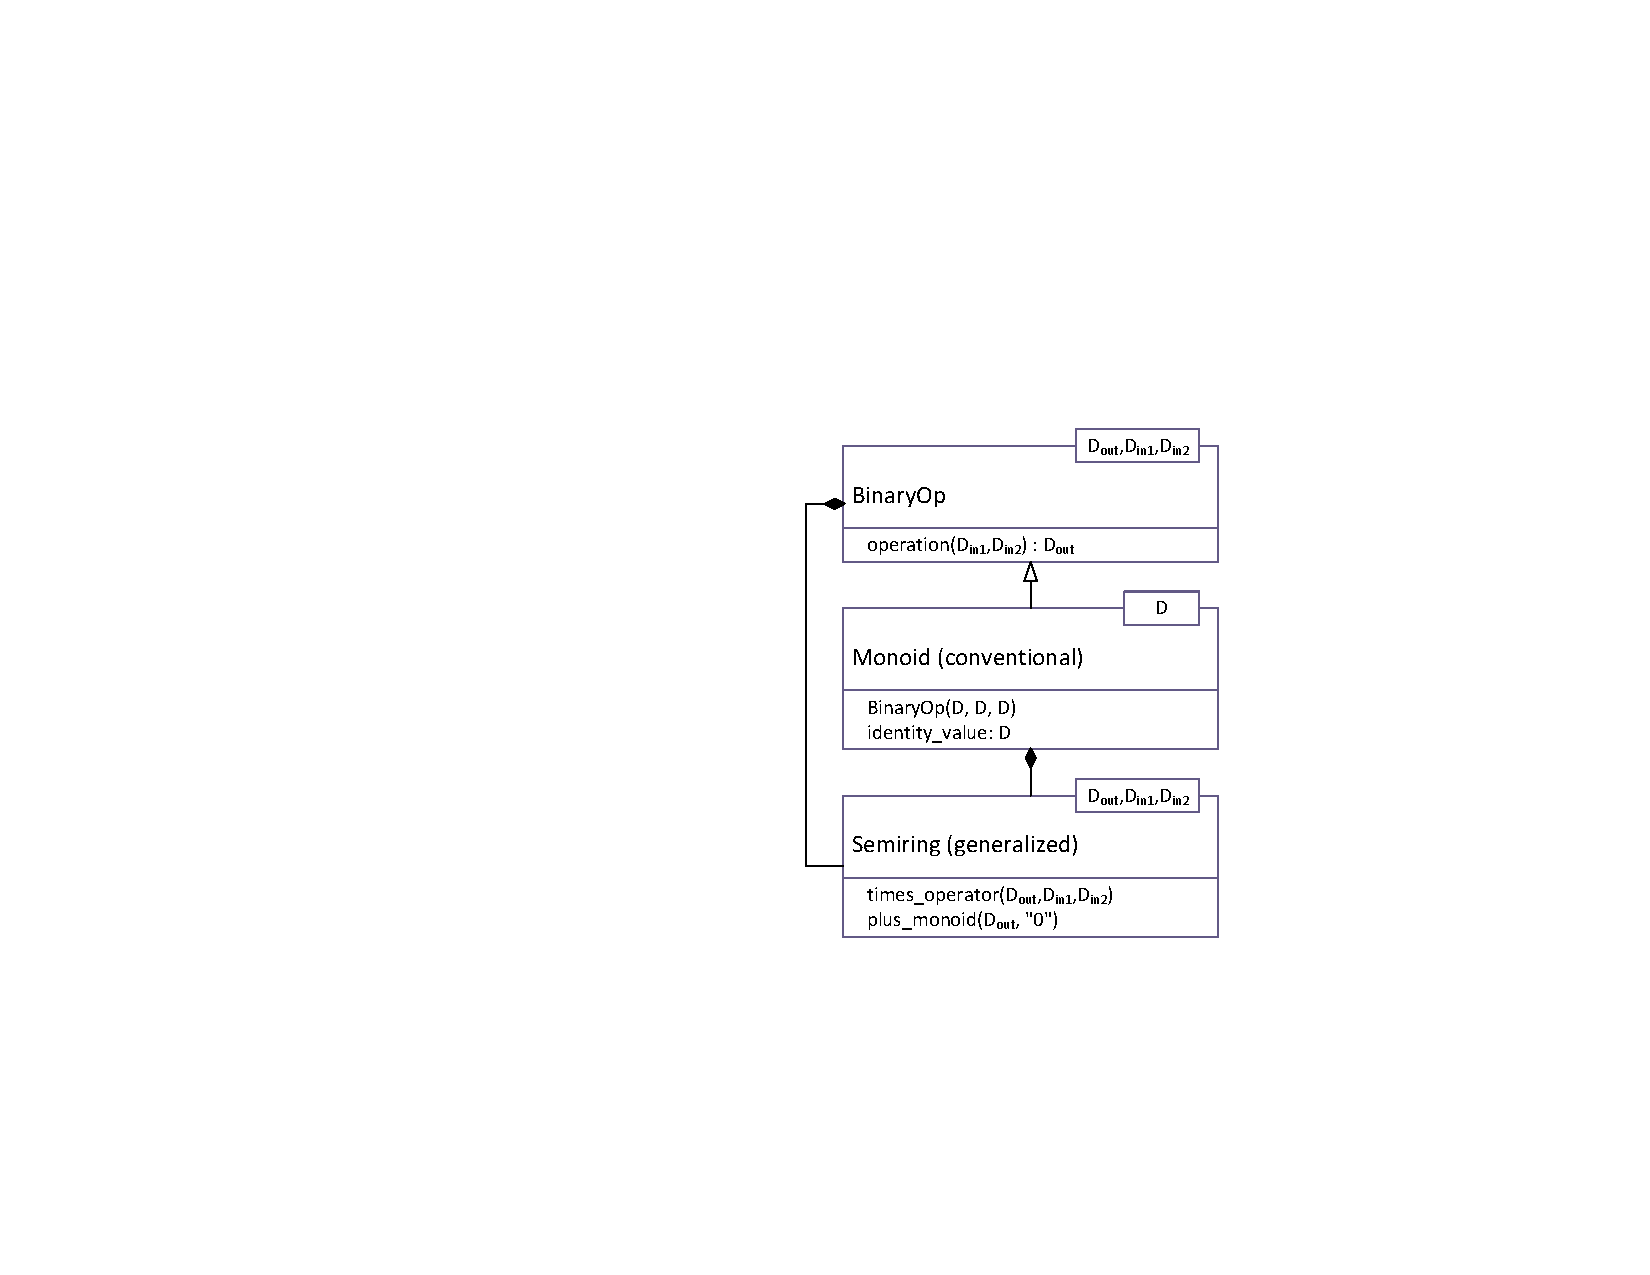
\includegraphics[width=1.0\linewidth,trim=3in 2in 0.5in 2in]{Algebra_Hierarchy_v2_1.pdf}
    \end{center}
    \caption{Hierarchy of algebraic object classes in GraphBLAS. GraphBLAS 
    semirings consist of a conventional monoid with one domain for the addition 
    function, and a binary operator with three domains for the multiplication function.}
    \label{Fig:AlgebraHierarchy}
    \hrule
\end{figure}

\section{Scalars \scott{NEW CONTENT}}
\label{Sec:Scalars}

A \emph{GraphBLAS scalar}, $\scalar{s} = \langle D, \{ \sigma \} \rangle$, is defined by
a domain $D$, and a set of zero or one \emph{scalar value}, $\sigma$, where $\sigma \in D$. 
We define $\mathbf{size}(\scalar{s}) = 1$ (constant), and
$\mathbf{L}(\scalar{s}) = \{ \sigma \}$. The set $\mathbf{L}(\scalar{s})$ is
called the \emph{contents} of the GraphBLAS scalar $\scalar{s}$. We also define 
$\mathbf{D}(\scalar{s}) = D$. Finally, $\mathbf{val}(s)$ is a 
reference to the scalar value, $\sigma$, if the GraphBLAS scalar is not empty, and is 
undefined otherwise.

\section{Vectors}
\label{Sec:Vectors}

A vector $\vector{v} = \langle D, N, \{ (i,v_i) \} \rangle$ is defined by
a domain $D$, a size $N>0$, and a set of tuples $(i,v_i)$ where $0 \leq
i < N$ and $v_i \in D$. A particular value of $i$ can appear at
most once in $\vector{v}$. We define $\mathbf{size}(\vector{v}) = N$ and
$\mathbf{L}(\vector{v}) = \{ (i,v_i) \}$. The set $\mathbf{L}(\vector{v})$ is
called the \emph{content} of vector $\vector{v}$. We also define the set
$\vector{ind(\vector{v})} = \{ i : (i,v_i) \in \mathbf{L}(\vector{v}) \}$
(called the \emph{structure} of $\vector{v}$), and $\mathbf{D}(\vector{v})
= D$. For a vector $\vector{v}$, $\vector{v}(i)$ is a reference to $v_i$
if $(i,v_i) \in \mathbf{L}(\vector{v})$ and is undefined otherwise.

\section{Matrices}
\label{Sec:Matrices}

A matrix $\matrix{A} = \langle D, M, N, \{ (i,j,A_{ij}) \} \rangle$ is
defined by a domain $D$, its number of rows $M>0$, its number of columns
$N>0$, and a set of tuples $(i,j,A_{ij})$ where $0 \leq i < M$, $0 \leq
j < N$, and $A_{ij} \in D$. A particular pair of values $i,j$ can
appear at most once in $\matrix{A}$. We define $\mathbf{ncols}(\matrix{A})
= N$,  $\mathbf{nrows}(\matrix{A}) = M$, and $\mathbf{L}(\matrix{A}) =
\{ (i,j,A_{ij}) \}$.  The set $\mathbf{L}(\matrix{A})$ is called the
\emph{content} of matrix $\matrix{A}$.  We also define the sets
$\vector{indrow(\matrix{A})} = \{ i : \exists (i,j,A_{ij}) \in
\matrix{A} \}$ and $\vector{indcol(\matrix{A})} = \{ j : \exists
(i,j,A_{ij}) \in \matrix{A} \}$.  (These are the sets of nonempty
rows and columns of $\matrix{A}$, respectively.)  The \emph{structure}
of matrix $\matrix{A}$ is the set $\mathbf{ind}(\matrix{A}) = \{ (i,j) :
(i,j,A_{ij}) \in \mathbf{L}(\matrix{A}) \}$, and $\mathbf{D}(\matrix{A}) = D$.
For a matrix $\matrix{A}$, $\matrix{A}(i,j)$ is a reference to $A_{ij}$
if $(i,j,A_{ij}) \in \mathbf{L}(\matrix{A})$ and is undefined otherwise.

If $\matrix{A}$ is a matrix and $0 \leq j < N$, then $\matrix{A}(:,j)
= \langle D, M, \{(i,A_{ij}) : (i,j,A_{ij}) \in \mathbf{L}(\matrix{A})
\} \rangle$ is a vector called the $j$-th \emph{column}
of $\matrix{A}$. Correspondingly, if $\matrix{A}$ is a matrix and
$0 \leq i < M$, then $\matrix{A}(i,:) = \langle D, N, \{(j,A_{ij}) :
(i,j,A_{ij}) \in \mathbf{L}(\matrix{A}) \} \rangle$ is a vector called
the $i$-th \emph{row} of $\matrix{A}$.

Given a matrix $\matrix{A} = \langle D, M, N, \{ (i,j,A_{ij}) \} \rangle$,
its \emph{transpose} is another matrix $\matrix{A}^T = \langle D, N, M, \{
(j,i,A_{ij}) : (i,j,A_{ij}) \in \mathbf{L}(\matrix{A}) \} \rangle$.

\section{Masks}
\label{Sec:Masks}

The GraphBLAS C API defines an opaque object called a \emph{mask}.  The mask
is used to control how computed values are stored in the output from a method. 
The mask is an \emph{internal} opaque object; that is, it is never exposed as a variable
within an application. 

The mask is formed from objects input to the method that uses 
the mask.  For example, a GraphBLAS method may be called with a matrix as the mask
parameter.   The internal mask object is constructed from the input matrix in one
of two ways.  In the default case, an element of the mask is created for each 
tuple that exists in the matrix for which the value of the tuple cast to Boolean 
evaluates to {\tt true}.  Alternatively, the user can specify {\em structure}-only behavior where
an element of the mask is created for each tuple that exists in the matrix 
{\em regardless} of the value stored in the input matrix.
\scott{STRUCTURE\_ONLY changes.}

The internal mask object can be either a one- or a two-dimensional construct.  One- and
two-dimensional masks, described more formally below, are similar to
vectors and matrices, respectively, except that they have structure
(indices) but no values.  When needed, a value is implied for the elements of a 
mask with an implied value of {\tt true} for elements that exist 
and an implied value of {\tt false} for elements that do not exist (\ie,
the locations of the mask that do not have a stored value imply a value of {\tt false}).
Hence, even though a mask does not contain any values, it can be 
considered to imply values from a Boolean domain.

A one-dimensional mask $\vector{m} = \langle N, \{ i \} \rangle$ is
defined by its number of elements $N>0$, and a set $\mathbf{ind}(\vector{m})$
of indices $\{ i \}$ where $0 \leq i < N$.  A particular value of $i$ can
appear at most once in $\vector{m}$. We define $\mathbf{size}(\vector{m})
= N$. The set $\mathbf{ind}(\vector{m})$ is called the \emph{structure} of mask $\vector{m}$.

A two-dimensional mask $\matrix{M} = \langle M, N, \{ (i,j) \}
\rangle$ is defined by its number of rows $M>0$, its number of
columns $N>0$, and a set $\mathbf{ind}(\matrix{M})$ of tuples $(i,j)$
where $0 \leq i < M$, $0 \leq j < N$.   A particular pair of values
$i,j$ can appear at most once in $\matrix{M}$.  We define
$\mathbf{ncols}(\matrix{M}) = N$, and $\mathbf{nrows}(\matrix{M}) = M$.
We also define the sets $\vector{indrow(\matrix{M})} = \{ i : \exists
(i,j) \in \mathbf{ind}(\matrix{M}) \}$ and $\vector{indcol(\matrix{M})}
= \{ j : \exists (i,j) \in \mathbf{ind}(\matrix{M}) \}$.  These are
the sets of nonempty rows and columns of $\matrix{M}$, respectively.
The set $\mathbf{ind}(\matrix{M})$ is called the \emph{structure} of mask $\matrix{M}$.

One common operation on masks is the \emph{complement}.
For a one-dimensional mask $\vector{m}$ this is denoted as
$\neg\vector{m}$. For a two-dimensional masks, this is denoted as
$\neg\matrix{M}$.  The complement of a one-dimensional
mask $\vector{m}$ is defined as $\mathbf{ind}(\neg\vector{m}) = \{i : 0
\leq i < N, i \notin \mathbf{ind}(\vector{m}) \}$.  It is the set of all
possible indices that do not appear in $\vector{m}$.  The 
complement of a two-dimensional mask $\matrix{M}$ is defined as the set
$\mathbf{ind}(\neg\matrix{M}) = \{(i,j)$ : $0 \leq i < M$, $0 \leq j < N$,
$(i,j) \notin \mathbf{ind}(\matrix{M}) \}$.  It is the set of all possible
indices that do not appear in $\matrix{M}$.

\section{Descriptors}
\label{Sec:Descriptors}

Descriptors are used to modify the behavior of a GraphBLAS method.
When present in the signature of a method, they appear as the last
argument in the method.  Descriptors specify how the other input arguments
corresponding to GraphBLAS collections -- vectors, matrices, and masks
-- should be processed (modified) before the main operation of a method
is performed.

The descriptor is a lightweight object.  It is composed of (\emph{field},
\emph{value}) pairs where the \emph{field} selects one of the GraphBLAS objects
from the argument list of a method and the \emph{value} defines the
indicated modification associated with that object.  For example,
a descriptor may specify that a particular input matrix needs to be
transposed or that a mask needs to be complemented (defined
in Section~\ref{Sec:Masks}) before using it in the operation.

For the purpose of constructing descriptors, the arguments of a method
that can be modified are identified by specific field names. The output
parameter (typically the first parameter in a GraphBLAS method) is
indicated by the field name, {\sf GrB\_OUTP}.  The mask is indicated
by the {\sf GrB\_MASK} field name. The input parameters corresponding
to the input vectors and matrices are indicated by {\sf GrB\_INP0}
and {\sf GrB\_INP1} in the order they appear in the signature of the
GraphBLAS method.  The descriptor is an opaque object and hence we do not
define how objects of this type should be implemented.   When referring to
(\emph{field}, \emph{value}) pairs for a descriptor, however, we often use the informal
notation {\sf desc[GrB\_Desc\_Field].GrB\_Desc\_Value} without implying
that a descriptor is to be implemented as an array of structures (in fact,
field values can be used in conjunction with multiple values that are composable).
We summarize all types, field names, and values used with descriptors
in Table~\ref{Tab:DescTypeLiterals}.

\begin{table}
\hrule
\begin{center}
\caption{Descriptors are GraphBLAS objects passed as arguments to Graph\_BLAS 
operations to modify other GraphBLAS objects in the operation's argument list.
A descriptor, {\sf desc}, has one or more (\emph{field}, \emph{value}) pairs indicated 
as  {\sf desc[GrB\_Desc\_Field].GrB\_Desc\_Value}. In this table, we define all types and literals used
with descriptors.}
\label{Tab:DescTypeLiterals}

\vspace{1\baselineskip}
(a) Types used with GraphBLAS descriptors.
\vspace{1\baselineskip}

\begin{tabular}{l|l}
Type			& Description \\ \hline
{\sf GrB\_Descriptor}     &  Type of a GraphBLAS descriptor object. \\
{\sf GrB\_Desc\_Field}              &  Type of a descriptor field. \\
{\sf GrB\_Desc\_Value}             &  Type of a descriptor field's value. \\
\end{tabular}

\vspace{1\baselineskip}
(b) Descriptor field names of type {\sf GrB\_Desc\_Field}.
\vspace{1\baselineskip}

\begin{tabular}{l|l}
Field name          & Description \\ \hline
{\sf GrB\_OUTP} &  Field name for the output GraphBLAS object. \\
{\sf GrB\_INP0}   &  Field name for the first input GraphBLAS object. \\
{\sf GrB\_INP1}   &  Field name for the second input  GraphBLAS object. \\
{\sf GrB\_MASK} &  Field name for the mask GraphBLAS object. \\\
\end{tabular}

\vspace{1\baselineskip}
(c) Descriptor field values of type {\sf GrB\_Desc\_Value}.
\scott{STRUCTURE\_ONLY changes.}
\vspace{1\baselineskip}

\begin{tabular}{l|l}
Field Value          & Description \\ \hline
{\sf GrB\_STRUCTURE} &  The write mask is constructed from the structure (pattern of stored \\
                     &  values) of the associated object. The stored values are not examined.\\
{\sf GrB\_COMP}      &  Use the complement of the associated object. When combined \\ 
                     &  with {\sf GrB\_STRUCTURE}, the complement of the structure of the associated \\
                     &  object is used without evaluating the values stored.\\
{\sf GrB\_SCMP}      &  Use the complement of the associated object. When combined \\ 
                     &  with {\sf GrB\_STRUCTURE}, the complement of the structure of the associated \\
             &  object is used without evaluating the values stored. {\color{red} This field value} \\
		     &  {\color{red} is currently deprecated in favor of {\sf GrB\_COMP} above, and may be} \\
		     &  {\color{red} removed in future versions of this API.} \\
{\sf GrB\_TRAN}      &  Use the transpose of the associated object.\\
{\sf GrB\_REPLACE}   &  Clear the output object before assigning computed values.\\
\end{tabular}
\end{center}
\hrule
\end{table}

In the definitions of the GraphBLAS methods, we often refer to the
\emph{default behavior} of a method with respect to the action of a
descriptor.   If a descriptor is not provided or if the value associated
with a particular field in a descriptor is not set, the default behavior
of a GraphBLAS method is defined as follows:
\begin{itemize}
\item Input matrices are not transposed.
\item The mask is used, as is, without complementing, and stored values are examined to 
determine whether they evaluate to {\tt true} or {\tt false}.\scott{STRUCTURE\_ONLY changes.}

\item Values of the output object that are not directly modified by the operation are preserved.
\end{itemize}

GraphBLAS specifies a set of pre-defined descriptors. Their identifiers
and the corresponding set of (field,value) pairs for that
identfier are shown in Table~\ref{Tab:DefaultDescriptors}.

\newcommand{\grboutp}{{\sf GrB\_OUTP}}
\newcommand{\grbmask}{{\sf GrB\_MASK}}
\newcommand{\grbinp}[1]{{\sf GrB\_INP#1}}
\newcommand{\grbreplace}{{\sf GrB\_REPLACE}}
\newcommand{\grbstructure}{{\sf GrB\_STRUCTURE}}
\newcommand{\grbscmp}{{\sf GrB\_COMP}}

\newcommand{\grbrepl}{{\sf GrB\_REPLACE}}
\newcommand{\grbstrc}{{\sf GrB\_STRUCTURE}}
\newcommand{\grbcomp}{{\sf GrB\_COMP}}
\newcommand{\grbtran}{{\sf GrB\_TRAN}}

\begin{table}[htbp]
    \hrule
    \begin{center}
	\caption{Pre-defined GraphBLAS descriptors. The list includes
	all possible descriptors, according to the current standard.  Columns list the
    possible fields and entries list the value(s) associated with those fields for
    a given descriptor.}
	\label{Tab:DefaultDescriptors}
~\\
	\begin{small}

        \begin{tabular}{l|llll} 
        Identifier          & {\sf GrB\_OUTP} & {\sf GrB\_MASK} & {\sf GrB\_INP0} & {\sf GrB\_INP1}  \\ \hline
        {\sf GrB\_NULL}     &    --    &    --    &    --    &    --    \\
        {\sf GrB\_DESC\_T1}       &    --    &    --    &    --    & \grbtran \\
        {\sf GrB\_DESC\_T0}       &    --    &    --    & \grbtran &    --    \\
        {\sf GrB\_DESC\_T0T1}     &    --    &    --    & \grbtran & \grbtran \\
        {\sf GrB\_DESC\_C}        &    --    & \grbcomp &    --    &    --    \\
        {\sf GrB\_DESC\_S}        &    --    & \grbstrc &    --    &    --    \\
        {\sf GrB\_DESC\_CT1}      &    --    & \grbcomp &    --    & \grbtran \\
        {\sf GrB\_DESC\_ST1}      &    --    & \grbstrc &    --    & \grbtran \\
        {\sf GrB\_DESC\_CT0}      &    --    & \grbcomp & \grbtran &    --    \\
        {\sf GrB\_DESC\_ST0}      &    --    & \grbstrc & \grbtran &    --    \\
        {\sf GrB\_DESC\_CT0T1}    &    --    & \grbcomp & \grbtran & \grbtran \\
        {\sf GrB\_DESC\_ST0T1}    &    --    & \grbstrc & \grbtran & \grbtran \\
        {\sf GrB\_DESC\_SC}       &    --    & \grbstrc, \grbcomp &    --    &    --    \\
        {\sf GrB\_DESC\_SCT1}     &    --    & \grbstrc, \grbcomp &    --    & \grbtran \\
        {\sf GrB\_DESC\_SCT0}     &    --    & \grbstrc, \grbcomp & \grbtran &    --    \\
        {\sf GrB\_DESC\_SCT0T1}   &    --    & \grbstrc, \grbcomp & \grbtran & \grbtran \\
        {\sf GrB\_DESC\_R}        & \grbrepl &    --    &    --    &    --    \\
        {\sf GrB\_DESC\_RT1}      & \grbrepl &    --    &    --    & \grbtran \\
        {\sf GrB\_DESC\_RT0}      & \grbrepl &    --    & \grbtran &    --    \\
        {\sf GrB\_DESC\_RT0T1}    & \grbrepl &    --    & \grbtran & \grbtran \\
        {\sf GrB\_DESC\_RC}       & \grbrepl & \grbcomp &    --    &    --    \\
        {\sf GrB\_DESC\_RS}       & \grbrepl & \grbstrc &    --    &    --    \\
        {\sf GrB\_DESC\_RCT1}     & \grbrepl & \grbcomp &    --    & \grbtran \\
        {\sf GrB\_DESC\_RST1}     & \grbrepl & \grbstrc &    --    & \grbtran \\
        {\sf GrB\_DESC\_RCT0}     & \grbrepl & \grbcomp & \grbtran &    --    \\
        {\sf GrB\_DESC\_RST0}     & \grbrepl & \grbstrc & \grbtran &    --    \\
        {\sf GrB\_DESC\_RCT0T1}   & \grbrepl & \grbcomp & \grbtran & \grbtran \\
        {\sf GrB\_DESC\_RST0T1}   & \grbrepl & \grbstrc & \grbtran & \grbtran \\
        {\sf GrB\_DESC\_RSC}      & \grbrepl & \grbstrc, \grbcomp &    --    &    --    \\
        {\sf GrB\_DESC\_RSCT1}    & \grbrepl & \grbstrc, \grbcomp &    --    & \grbtran \\
        {\sf GrB\_DESC\_RSCT0}    & \grbrepl & \grbstrc, \grbcomp & \grbtran &    --    \\
        {\sf GrB\_DESC\_RSCT0T1}  & \grbrepl & \grbstrc, \grbcomp & \grbtran & \grbtran \\
        \end{tabular}
	\end{small}

    \end{center}
    \hrule
\end{table}

